%%%%%%%%%%%%%%%%%%%%%%%%%%%%%%%%%%%%%%%%%%%%%%%%%%%%
%%%%%%% Verslag Tinlab Advanced Algoritms %%%%%%%
%%%%%%%%%%%%%%%%%%%%%%%%%%%%%%%%%%%%%%%%%%%%%%%%%%%%

\documentclass{article}
\usepackage{graphicx}
\usepackage[font=small,labelfont=bf]{caption}
\usepackage[dutch]{babel}

\usepackage[a4paper, total={6in, 8in}]{geometry}

%Includes "References" in the table of contents
\usepackage[nottoc]{tocbibind}

% libraries for use of Liveness operator
\usepackage{tikz}
\usetikzlibrary{decorations.pathmorphing}
\usepackage{amssymb}

\begin{document}

	\sffamily
	%%%%%%% Front page %%%%%%%
	%%%%%%%%%%%%%%%%%%%%%%%%%%%%%%%%%%%%%%%%%%%%%%%%%%%%
	
	\begin{titlepage}
	
		\centering
		  \vfill
		  {\bfseries\Huge
		    Verslag Tinlab Advanced Algorithms \\
		      \vskip2cm
		    }
		    {\bfseries\Large
		      Thijs Dregmans\\
		    }
		    {
		      \bfseries\normalsize
		      1024272\\
		      \vskip1cm
		      \today\\
		  }    
		  \vfill
		  
\includegraphics[width=4cm]{logohr.png} % also works with logo.pdf
		  \vfill
		  \vfill
	    
	\end{titlepage}
	
	\newpage
	
	%%%%%%% Table of Content %%%%%%%
	%%%%%%%%%%%%%%%%%%%%%%%%%%%%%%%%%%%%%%%%%%%%%%%%%%%%
	
	\tableofcontents
	
	\newpage
	
	%%%%%%% Inleiding %%%%%%%
	%%%%%%%%%%%%%%%%%%%%%%%%%%%%%%%%%%%%%%%%%%%%%%%%%%%%
	
	\section{Inleiding}
	
	Voor de cursus 'Advanced Algorithms' van de opleiding Technische Informatica heb ik het volgende verslag geschreven. Het is een verwerking en samenvatting van de lesstof. Het dient zowel als naslagwerk voor mijzelf, als het aantonen van het behalen van de leerdoelen voor de cursus. \\
	
Het Tinlab begon met het behandelen van het probleem van specificeren van requirements. Dit is alle design domeinen een groot probleem. Goede requirements definieren is een hoofdpijn dossier. We hebben naar systemen gekeken door het vier variabelen model. Vervolgens zijn een aantal rampen bekeken om dit model in de praktijk te gebruiken om uitspraken te doen over het falen van systemen.  \\

	[geef een samenvatting van de cursus]
	
	\newpage
	
	%%%%%%% Requirements %%%%%%%
	%%%%%%%%%%%%%%%%%%%%%%%%%%%%%%%%%%%%%%%%%%%%%%%%%%%%
	
	\section{Requirements}
	
	Requirements zijn eisen die gesteld worden aan een systeem. Er zijn veel verschillende soorten requirements. Axel van Lamsweerde schrijft in zijn boek 'Requirements Engineering' over een aantal: \cite{Lamsweerde2009Requirements}

	\begin{itemize}
		\item Functional requirements

			Functional requirements zeggen iets over hoe het systeem zich moet gedragen.

		\item Non-functional requirements

			Non-functional requirements werken verder uit hoe functional requirements vervuld moeten worden.

		\item Quality requirements

			Quality requirements stellen eisen aan 'hoe goed' het systeem de functional requirements moet vervullen. Denk hierbij aan veiligheid, integeriteit, beschikbaarheid en betrouwbaarheid van informatie. \par

		\item Compliance requirements
	
		Compliance requirements zeggen iets over de wettelijke (juridische) kaders het systeem dient te handhaven.

		\item Architectural requirements
	
		Architectural requirements geven meer informatie over hoe het systeem er uit moet zien, in de architectuur.

		\item Development requirements

		Development requirements werken uit welke eisen gesteld worden aan de ontwikkeling van het systeem. Dit kan bijvoorbeeld gaan over het budget en eventuele deadlines. \par

	\end{itemize}

	In dit Tinlab wordt onderscheid gemaakt tussen twee verschillende types requirements:

	\begin{enumerate}
		\item System requirements
		\item Software requirements
	\end{enumerate}

	System requirements doen uitspraken over de wereld en de fenomenen in de wereld - of ze spreken over een doel dat bereikt moet worden. Software requirements doen uitspraken over fenomenen in de machine - of over doelen die de machine moet bereiken. \par

	Software kan van zichzelf niet communiceren met de buitenwereld. Een systeem communiceert met de buitenwereld middels sensoren en actuatoren. \par
		
		%%%%%%%%%%%%%%%%%%%%%%%%%%%%%%%%%%%%%%%%%%%%%%%%%%%%
		\subsection{Requirements specificeren}
		
		Het proces waarmee requirements worden 'ontdekt' wordt "Requirements elicitation" genoemd. Lamsweerde identificeert in hoofdstuk 2 van zijn boek verschillende methodes voor het ontdekken van requirements:

		\begin{enumerate}
			\item Achtergrond studie
			\item Statistisch onderzoek
			\item Gebruik van prototypes
			\item Mogelijke scenario's 
			\item Enquetes
			\item Interviews
			\item Observaties
			\item Brainstorm sessies
		\end{enumerate}

		Het is vrijwel onvermijdelijk dat requirements strijdig zijn. Er kan bijvoorbeeld een development requirement zijn die zegt dat het product voor een bepaalde deadline af moet zijn, terwijl een andere - bijvoorbeeld architectural - requirement zegt dat een bepaalde architectuur gevolgt moet worden. Het kan zijn, dat het implementeren van zo'n architectuur niet haalbaar is binnen de deadline. In zo'n geval is een 'trade-off' noodzakelijk. De stakeholders komen dan bijvoorbeeld overeen dat een dergelijke architectuur dan achterwege gelaten kan worden. Bij dit proces is het van belang dat de eisen vanuit verschillende invalshoeken bekeken worden, dat de redenen achter de eisen meegenomen worden en dat gekeken wordt naar mogelijke alternatieve oplossingen. \par
		
		%%%%%%%%%%%%%%%%%%%%%%%%%%%%%%%%%%%%%%%%%%%%%%%%%%%%
		\subsection{Het vier variabelen model}
		
		Een handige manier om systemen te conceptualiseren is het vier variabelen model. Het gebruik van het vier variabelen model gaat terug naar 1978. Het is voornamelijk handig bij het analyseren en ontwerpen van veiligheidskritieke systemen. \cite{patcas2014system} Zie Figuur 1 voor een uitwerking van dit model. \par
		
		\begin{center}
			\begin{minipage}{0.48\linewidth}
				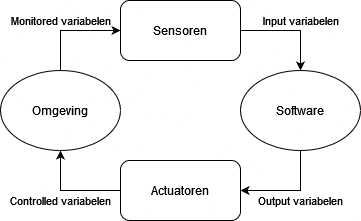
\includegraphics[width=\linewidth]{4variabelen.png}
				\captionof{figure}{4 variabelen model}
			\end{minipage}
			\hfill
		\end{center}

		Dit model komt vooruit het idee van twee werelden die overlappen. Er is een tastbare wereld, met verschillende fenomenen. Deze wereld is de werld waarin wij leven. In deze wereld zijn problemen die wij willen oplossen met systemen. Zo'n systeem is geen onderdeel van de tastbare wereld. Het systeem is een wereld op zichzelf. Er wel enig overlap tussen de syteem-wereld en de tastbare wereld. Het overlap tussen deze werelden is de hardware, specifiek de sensoren en actuatoren. \par

		De systeem-wereld is de software. Deze wereld heeft in zichzelf geen enkel idee van het bestaan van een ander wereld. De tastbare wereld is de omgeving waarin de het systeem functioneert (of moet functioneren). Ook deze wereld heeft geen idee van de werking van de ander. Dit is ook niet mogelijk of belangrijk, zolang de sensoren en actuatoren naar behoren functioneren. \par

		De 4 verschillende delen van de van de werelden - omgeving, sensoren, software en actuatoren - communiceren met elkaar met behulp van variabelen. \par
	
		System requirements definiëren de relaties tussen de monitored variabelen en de controlled variabelen:

		\[ SysReq \subseteq M \times C\]

		Software requirements definiëren de relaties tussen de input variabelen en de output variabelen:

		\[ SoftReq \subseteq I \times O \]
		
			%%%%%%%%%%%%%%%%%%%%%%%%%%%%%%%%%%%%%%%%%%%%%%%%%%%%
			\subsubsection{Monitored variabelen}
			
			Monitored variabelen zijn de variabelen uit de wereld die door de sensoren wordt waargenomen en gemeten. \par
			
			Ter voorbeeld, een Monitored variabele kan de temperatuur zijn. De omgeving is bijvoorbeeld binnenshuis, bij iemand thuis. De sensor is een temperatuursensor. De sensor meet de waarde/variabele. \par
			
			%%%%%%%%%%%%%%%%%%%%%%%%%%%%%%%%%%%%%%%%%%%%%%%%%%%%
			\subsubsection{Input variabelen}
			
			Input variabelen zijn de variabelen die door de sensor worden doorgegeven aan de software. \par

			In het voorbeeld van de temperatuursensor, heeft de temperatuursensor de Monitored variabele omgezet in een reeks bits. Deze bits worden door de sensor naar de microcontroller gestuurd. Voor de software die op de microcontroller staat, is dit de input. In het syteem geldt deze bits als Input variabele. \par
			
			%%%%%%%%%%%%%%%%%%%%%%%%%%%%%%%%%%%%%%%%%%%%%%%%%%%%
			\subsubsection{Output variabelen}
			
			Output variabelen zijn de variabelen die door de software worden geproduceerd en worden doorgegeven aan de actuatoren. \par

			In het voorbeeld, heeft de software van de microcontroller de temperatuur - in de vorm van een aantal bits - omgezet in een output. De output is in dit voorbeeld een instructie voor een warmte element om aan te gaan, indien de temperatuur onder een bepaalde waarde zakt. De instructie voor het warmte element is de output van de software, en daarom - in dit voorbeeld - de Output variabele. \par

			%%%%%%%%%%%%%%%%%%%%%%%%%%%%%%%%%%%%%%%%%%%%%%%%%%%%
			\subsubsection{Controlled variabelen}

			Controlled variabelen zijn de variabelen in de omgeving die door de actuatoren worden beïnvloed, of 'Controlled'. \par

			In dit voorbeeld, is er door de microcontroller een instructie gegeven aan het warmte element. De microcontroller bevat de software en het warmte element is de actuator. Door de instructie van de software gaat het warmte element aan, en wordt het warmer in huis. De temperatuur stijgt. De Controlled variabele in dit voorbeeld is de temperatuur. \par

			
			In dit voorbeeld is de Controlled variabele en de Monitored variabele dezelfde variabele, maar dat hoeft niet zo te zijn. Men kan in plaats van een warmte element, ook een lampje aansluiten, die dan aan zou gaan bij een bepaalde temperatuur. In dit geval zou de Controlled variabele het licht van het lampje zijn. \par

		%%%%%%%%%%%%%%%%%%%%%%%%%%%%%%%%%%%%%%%%%%%%%%%%%%%%
		\subsection{Het zes variabelen model}

		Bij gebruik van het vier variabelen model, kunnen de ontwerpkeuzes die betrekking hebben op concretiseren van de context, niet gebruikt worden om bij het toepassen van het systeem in een nieuwe omgeving. Dit is het geval omdat de context - in andere woorden, de omgeving - één van de variabelen is, terwijl die vaak nog niet goed is gedefinieerd. Het zes variabelen model tracht dit te verhelpen door twee extra variabelen toe te voegen: \par

		\begin{enumerate}
			\setcounter{enumi}{4}
			\item Referenced variable
			\item Desired variable
		\end{enumerate}

			%%%%%%%%%%%%%%%%%%%%%%%%%%%%%%%%%%%%%%%%%%%%%%%%%%%%
			\subsubsection{Gerefereerde variabelen}
			
			Gerefereerde variabelen zijn de variabelen uit de wereld die door de sensoren wordt waargenomen en gemeten. Deze definitie is gelijk aan die van de Monitered variabelen. Een van de aannames die het model heeft, is dat deze gelijk zijn. Het is echter nodig om onderscheid te maken om een relatie "Real-World requirements" te kunnen introduceren. Deze relatie is de relatie tussen de Gerefereerde variabelen en de Verlangde variabelen. \par

			De Gerefereerde variabelen zijn de variabelen in de 'echte wereld', zoals de wereld is ook zonder dat het systeem werkt - of zonder dat het systeem bestaat. De Monitored variabelen zijn de variabelen die door het systeem observeert worden. Er kan pas iets geobserveerd worden, als er een systeem is om te observeren. Zonder systeem kan je dus technisch gezien geen Monitered variabelen definieren. Vandaar het onderscheid. \par
			
			%%%%%%%%%%%%%%%%%%%%%%%%%%%%%%%%%%%%%%%%%%%%%%%%%%%%
			\subsubsection{Verlangde variabelen}
			
			Verlangde variabelen zijn de variabelen in de omgeving die door de actuatoren worden beïnvloed. Deze definitie is gelijk aan die van de Controlled variabelen. Dit is echter nodig om de relatie "Expectation" - het verwachte resultaat - tussen de Verlangde variabelen en de Controlled variabelen te definieren. \par

			De Verlangde variabelen zijn de variabelen in de 'echte wereld', zoals de wereld is ook zonder dat het systeem werkt - of zonder dat het systeem bestaat. De Controlled variabelen zijn de variabelen die door het systeem beïnvloed worden. Er kan pas iets beïnvloed worden, als er een systeem is om te beïnvloeden. Zonder systeem kan je dus technisch gezien geen Beïnvloede variabelen definieren. Vandaar het onderscheid. \cite{icsoft-pt16} \par
		
		%%%%%%%%%%%%%%%%%%%%%%%%%%%%%%%%%%%%%%%%%%%%%%%%%%%%
		\subsection{Rampen}
		
		De werking en uitleg van het vier variabelen model wordt gedemonstreerd aan de hand van een aantal rampen. \par
		
			%%%%%%%%%%%%%%%%%%%%%%%%%%%%%%%%%%%%%%%%%%%%%%%%%%%%
			\subsubsection{Therac-25}

				\paragraph{Beschrijving}

				In de Verenigde Staten vonden in de jaren 80 een serie ongelukken plaats, waarbij verschillende patienten een dodelijke dosis straling kreeg toegediend met de Therac-25. Anderen raakten zwaar-gewond. De Therac-25 verschilde met zijn voorloper - de Therac-20 - op een belangrijke manier. De Therac-20 is ook een computergestuurde machine, maar heeft ook hardware veiligheidsmaatregelen. In de Therac-25 zijn deze hardware veiligheidsmaatregelen verdwenen en vervangen door software die hetzelfde effect zouden moeten hebben. \cite{thomas1994story} \par

				\paragraph{Datum en plaats}

				De ongelukken vonden plaats in de Verenigde Staten, tussen 1985 en 1987. \par

				\paragraph{Oorzaak}

				De zes ongelukken zijn aan verschillende zaken te wijden. Leveson en Turner schrijven uitgebreid over de oorzaken. \cite{274940} \par

				\begin{itemize}
					\item De Therac-25 verwijderde de veiligheidshardware die wel aanwezig was op de Therac-20. \par
						
						Dit is een ontwerp fout. In het licht van het vier-variabelen model, zou dit ofwel een Software fout, ofwel een Actuator fout kunnen zijn. Men zou kunnen beargumenteren dat dit een Software fout is omdat de hardware veiligheidsmaatregelen die zijn verwijderd, in de software zouden moeten terugkomen. Dit is niet het geval. Men zou ook kunnen beargumenteren dat het hier gaat om een falende Actuator, omdat de benodigde veiligheidshardware niet aanwezig is (volgens het ontwerp). \par

					\item De Therac-25 had cryptisch foutmelding, die vaak enkel het woord "malfunction" bevatten, samen met een error code - een getal van 1 tot 64. Het was voor de gebruiker onduidelijk wat deze betekenden. Het was niet duidelijk of een dergelijke foutmelding de patient in gevaar kon brengen. Ook in de handleiding wordt niet gesproken over foutcodes. \par

						Men moet nooit een foutmelding negeren; zeker niet als men werkt met een machine die een levensgevaarlijke dosis kan toedienen aan machines. De vraag is of de medewerkers (die de Therac-25 gebruikte) te verwijten valt, dat ze de foutmeldingen negeerden. De onduidelijkheid van de betekenis van de foutmeldingen, zowel in de melding zelf als in de handleiding, is een fout aan de kant van de fabrikant. Dit is opnieuw een ontwerpfout. De machine had met de foutmelding een uitgebreide beschrijving van de fout moeten geven. Daarom is het een Software fout. \par

					\item De Therac-25 heeft 3 modi. Door een meganisch-draaiende schijf werd de installatie gereed gemaakt voor de juiste modus. Een sensor detecteerde of de schijf in de juiste positie stond. Deze gaf een 3 bits waarde terug. Een kleine foute elektronische fout kan een incorrect waarde teruggeven, waardoor een patient een overdosis kan krijgen. \par

						Omdat het hier gaat om een elektronische fout (kortsluiting), die voor een incorrecte waarde zorgt, gaat het hier om een Sensor fout. De sensor was onvoldoende bestendig tegen elektronische fouten, wat resulteerde in een foutieve waarde. \par

					\item De installatie gereed maken kost 8 seconden. Als de gebruiker kiest voor een bepaalde opstelling, dan wordt die gereed gemaakt. Als de gebruiker dan vervolgens nog voordat de installatie gereed is, de opstelling wijzigt, dan wordt dit niet opgemerkt. Op het scherm wordt de juiste opstelling getoond, maar in werkelijkheid is het systeem nog niet gereed. \par

						Als een modus is geselecteerd, dan begint het systeem de installatie gereed te maken. Het systeem houdt in de tussentijd niet bij of de daadwerkelijke modus verandert, als de gebruiker de geselecteerde modus verandert. Dit is een Software fout. De Therac-25 zou of het veranderen van de modus binnen 8 seconden niet moeten toestaan, of getoonde modus op het scherm ten alle tijden overeen moeten laten komen met de stand van het systeem. \par
				\end{itemize}
			
			%%%%%%%%%%%%%%%%%%%%%%%%%%%%%%%%%%%%%%%%%%%%%%%%%%%%
			\subsubsection{Vlucht 1951}
				\paragraph{Beschrijving}

Een vliegtuig van het type Boeing 737-800 van de Turkish Airlines storte in 2009 vlak voor het landen op Schiphol neer. Er waren 3 piloten, 4 mensen van het cabinepersoneel en 128 passagiers aan boord. Alle piloten, 1 persoon van het cabinepersoneel en 5 passagiers vonden door het ongeluk de dood. \par

				\paragraph{Datum en plaats}

					Het ongeluk vond plaats terwijl het vliegtuig op 25 februari 2009 aan het landen was op Schiphol, in Amsterdam. \par

				\paragraph{Oorzaak}

					Omdat het ongeval in Nederland plaatsvond, deed de Onderzoeksraad voor Veiligheid onderzoek. In mei 2010 kwam zij met haar eindverslag waaruit de volgende conclusies getrokken kunnen worden: \cite{OvV2009} \par
				
				\begin{itemize}

					\item De Boeing 737-800 heeft twee hoogtemeters aan boord. Er is sprake van een redundante functie: Standaard wordt de waarde van de linker sensor genomen. In het geval van een foutieve waarde, kan de rechter sensor gebruikt worden. In zo'n geval moet de waarde van de linker sensor wel als foutief gezien worden. In dit geval gaf de linker hoogtemeter een waarde van -8 voet, maar het systeem herkende dit niet als foutieve waarde. Het opvallende is dat de sensorwaarden van beide sensoren getoond werden op de displays. De piloten hebben echter het verschil niet - of te laat - opgemerkt.

					\item Op die bewuste dag, was de automatische piloot ingeschakeld. Het systeem gebruikte daarvoor de linker hoogtemeter, omdat deze waarde niet als foutief werd herkend. Omdat de automatische piloot de incorrecte waarde doorkreeg, begon het met het inzetten van de landing. Dit gebeurt normaal gesproken pas als het vliegtuig op een hoogte van minder dan 27 voet vliegt. Dit werd op het primaire display getoond met het codewoord 'RETARD' - de naam van deze modus. In deze modus wordt de snelheid flink verlaagd. De automatische piloot probeerde het vliegtuig in de lucht te houden, door de neus van het vliegtuig omhoog te duwen, om zo meer draagkracht te creeëren. Hier werd door de piloten niet op gereageerd.

					\item Toen het vliegtuig op een hoogte van 460 voet vloog, en het almaar snelheid en hoogte verloor, kwam het laatste waarschuwing signaal: De zogenaamde 'stick shaker'. In zo'n geval waarschuwt het vliegtuig de piloot dat het vliegtuig stagneert en alle draagkracht dreigt te verliezen door de stuurstok te schudden. De piloot moet de motoren op volle kracht zetten, en de stuurstok naar zich toe trekken.

					\item De eerste officier reageerde op de 'stick shaker' op de voorgeschreven wijze. Hij zette de motoren op volle kracht. De kapitein nam de besturing over, waardoor de reactie van de eerste officier overschreven werd. Dit heeft er waarschijnlijk toe geleid dat de motoren - door de automatische piloot die niet werd uitgeschakeld - weer terug schakelde naar het oude niveau, waarmee het vliegtuig doorging met stagneren. Op dat moment had het vliegtuig een hoogte van 350 voet. Dat bleek onvoldoende voor herstel.

			De Onderzoeksraad voor Veiligheid stelt dat het ongeluk is veroorzaakt door het niet-correct functioneren van de linker hoogtemeter. Deze zorgde ervoor dat de automatische piloot het vermogen te vroeg liet teruglopen, wat een te groot snelheidsverlies veroorzaakte.

			Met het oog op het het vier-variabelen model, lijkt hier sprake te zijn van een falende Sensor. Hoewel er een redundante sensor aanwezig was, is het van belang dat het systeem de foutieve sensorwaarde als zodanig herkent. Dat is hier niet gebeurt.

				\end{itemize}
			
			%%%%%%%%%%%%%%%%%%%%%%%%%%%%%%%%%%%%%%%%%%%%%%%%%%%%
			\subsubsection{Chernobyl}

				\paragraph{Beschrijving}

					Het ongeluk in Chernobyl staat bekend als één van de grootste radiologisch ongelukken in de geschiedenis. Het ongeval vond plaats tijdens een experiment waarbij de veiligheid in geval van het falen van een waterpomp. \cite{ragheb2010chernobyl} \par

				\paragraph{Datum en plaats}

					Het ongeluk vond plaats in noord Oekraine. Het was in die tijd onderdeel van de Sovjet-Unie. Op 26 april 1986 om 01:23 startte het experiment dat het ongeluk veroorzaakte. De gevolgen voor mens en milieu waren - en zijn nog steeds - desastreus. \cite{BERESFORD201677} \par

				\paragraph{Oorzaak}

				Het ongeluk is veroorzaakt door een 'positieve feedback loop' - een reactie die zichzelf kon voeden. Een gerenomeerde Sovjet wetenschapper - Valery Alekseyevich Legasov - zegt dat de ramp te wijden is aan (onkundig) menselijk handelen in combinatie met ontwerpfouten. \par

				In de reactor waren twee koelsystemen aanwezig. Het koelmiddel had als primaire functie om de neutronen - die tijdens de kernreactie vrijkomen - (deels) te absorberen, om zo een explosie te voorkomen. Een 'void' in het koelmiddel, laat de absorberende functie afnemen. Hierdoor neemt het aantal neutronen snel toe, en ook de energie van de reactor. Een hogere energie in de reactor laat het koelmiddel koken, wat zorgt voor stoomvorming. Dit zorgt op zijn beurt weer een vermindert aborberend effect. Dit zichzelf-versterkend effect heeft uiteindelijk tot het ongeluk geleid. \par

				In het licht van het vier variabelen model, is hier een fout in de omgeving. Door natuurkundige processen - die door in de omgeving aanwezige stoffen mogelijk werden gemaakt - kon de ramp plaats vinden. \par
			
			%%%%%%%%%%%%%%%%%%%%%%%%%%%%%%%%%%%%%%%%%%%%%%%%%%%%
			\subsubsection{Patriot Missile Defense System}

				\paragraph{Beschrijving}

					In de Golf Oorlog had de Verenigde Staten Patriot Missile Defense Systems gestationeerd in Dhahran, Saudi Arabia - haar bondgenoot. Door een systeemfout faalde het systeem in het neerhalen van een raket, wat resulteerde in 28 doden en honderden gewonden onder de gestationeerde Amerikaanse soldaten. \par

				\paragraph{Datum en plaats}

					Het noodlottig falen resulteerde in 28 doden en honderden gewonden op 25 februari 1991. Het systeem in kwestie was op dat moment gestationeerd in een Amerikaanse legerbasis in Dhahran, in Saoedi-Arabië. \cite{general1992patriot} \par

				\paragraph{Oorzaak}

					Het falen werd veroorzaakt door de computer die verantwoordelijk was van de berekeningen. Deze computer's interne klok had een kleine afwijking, waardoor na 100 uur op 100 uur en 0.3433 seconden stond. Naarmate de tijd vorderde, werd de foutmarge groter. \cite{skeel1992roundoff} Dit lijkt een klein detail, maar met de snelheden van de raketten die de het systeem moet onderscheppen, heeft dit grote invloed.  \par

					Twee weken voor het incident rapporteerde de Israëliers aan de Amerikanen dat wanneer het systeem 8 uur achtereen draaide, er onnauwkeurigheden optraden. De software werd hierop aangepast, om de nauwkeurigheid te verbeteren. Deze wijziging bereikte Dhahran echter pas de dag na het ongeluk - op 26 februari. \cite{general1992patriot} \par

					Met oog op het vier variabelen model, kan gesteld worden dat bij het Patriot Missile Defense System sprake was van een software fout. \par
			
			%%%%%%%%%%%%%%%%%%%%%%%%%%%%%%%%%%%%%%%%%%%%%%%%%%%%
			\subsubsection{Hitomi}

				\paragraph{Beschrijving}

					De 'Japan Aerospace Exploration Agency', kortweg JAXA, lanceerde in 2016 een raket met aan boord een satelliet. Deze sateliet 'Hitomi' moest de komende 10 jaar voorzien in gegevens die zouden moeten leiden tot nieuwe inzichten in de astronomie. Vijf weken na de lancering, raakten de Japanners de controle kwijt. Dit wordt gewijd aan een systeemfout. Het project kostte omgerekend zo'n 286 miljoen Amerikaanse Dollars.

				\paragraph{Datum en plaats}

					De lancering vond plaats op 17 februari 2016. Zo'n vijf weken later - op 26 maart om 3:01 's morgens - begon de Hitomi te draaien om een specifiek deel van het universum te observeren.

				\paragraph{Oorzaak}

					De Hitomi had een aantal systemen aan boord om de orientatie van de satelliet te detecteren en te handhaven. Bij deze ramp zijn twee van deze systemen betrokken: het 'star tracker' systeem en het systeem dat gebruik maakt van gyroscopen. \par

					 Tijdens het draaien, trad er een fout op in het standaard orientatie detectie systeem - de 'star tracker' - die ervoor zorgde dat de satelliet overschakelde naar de gyroscopen. Deze gyroscopen gaven aan een rotatie van 20 graden per uur te detecteren, hoewel de satelliet niet met die snelheid roteerde. De 'reaction wheels' werden in werking gesteld om de gedetecteerde rotatie tegen te gaan. \par

					Dit zorgde voor een positieve feedback. Door de reaction wheels ging de Hitomi sneller roteren. De satelliet had een veiligheidsmaatregel die moest voorkwam dat de satelliet te snel roteerde om zijn as. Voor het naar behoren functioneren van deze veiligheidsmaatregel was het echter nodig dat het orientatie detectie systeem naar behoren functioneerde. Omdat dit niet het geval was, faalde de veiligheidsmaatregel. \par

					Hierop schakelde het systeem een 'safe mode' in. Hierin werden motoren ingeschakeld, waarmee werd geprobeerd de rotatie te stoppen. Omdat er eerder een verkeerd commando is geupload naar de satelliet, werd de rotatie niet afgeremd, maar versneld. \par

					Ten minsten 10 onderdelen, waaronder de zonnepanelen die de Hitomi van stroom voorzagen, braken af. Sommige instrumenten aan boord waren al tientallen jaren in ontwikkeling. De JAXA hoopte op levenduur van 10 jaar. Hoewel de Hitomi niet compleet nutteloos is gebleken, had men op meer gehoopt. \cite{witze2016software} \par 

					De fout die deze ramp veroorzaakte zou - in het licht van het vier variabelen model - gecategoriseerd moeten worden als sensorfout. Het gaat hier immers om het foutief dectecteren van de orientatie en de rotatie, door de gyroscopen. Men zou overigens ook kunnen beargumenteren dat het hier gaat om een ontwerpfout die betrekking heeft op de omgeving. In de eerste plaats faalde het 'star track' systeem. Dit was een werd veroorzaakt door een glich die optrad wanneer de satelliet de 'South Atlantic Anomaly' passeerde. Op deze plek is de atmosfeer relatief laag, waardoor de satelliet op deze plek extra wordt blootgesteld aan straling. Deze glitch zou geen fataal probleem moeten zijn, maar heeft wel alle andere problemen mogelijk gemaakt. Er is in het ontwerp onvoldoende rekening gehouden met de extra straling waaraan het systeem wordt blootgesteld. \par
				
			%%%%%%%%%%%%%%%%%%%%%%%%%%%%%%%%%%%%%%%%%%%%%%%%%%%%
			\subsubsection{Mars Climate Orbiter}

				\paragraph{Beschrijving}

					De NASA lanceerde in 1998 de Mars Climate Orbiter. De formele naam is 'Mars Surveyor '98 Orbiter'. Het doel was om informatie te verzamelen over het klimaat en de atmosfeer op Mars. Daarnaast moest het apparaat dienen als tussenstation voor communicatie met de Mars Polar Lander - die ook onderdeel was van de missie. Tijdens deze missie waren er dus twee machines in bedrijf. De Mars Climate Orbiter (MCO) kwam tijdens het proces waarbij de satelliet in zijn baan wordt gebracht, te dicht bij de planeet wat resulteerde in een crash.

				\paragraph{Datum en plaats}

					De lancering van de de MCO was op 11 december 1998. Het ongeluk vond plaats in de atmosfeer van Mars tijdens het in zijn baan brengen van de satelliet op 23 september 1999.

				\paragraph{Oorzaak}

					Na de maanden lange reis kwam het object aan bij Mars, en kon de procedure begonnen worden waarmee de satelliet in zijn baan wordt gebracht. De MCO was asymetrisch van vorm. Door een kracht die ook wel Solar Radiation Pressure wordt genoemd, is de satelliet gaan draaien. Deze kracht wordt veroorzaakt door de zon, die straling afschiet op de satelliet die hierdoor uit zijn baan kan geraken. \cite{yousef2022balancing} Om voor deze SRP te corrigeren zijn flywheels tussen de 10 tot 14 keer vaker geactiveerd dan verwacht. Het systeem dat hiervoor verantwoordelijk was, is gebouwd door een andere partij dan de partij die de interface van het systeem gebruikte (in de software). Door onvoldoende testen en slechte communicatie kon het voorkomen dat het verantwoordelijke systeem Engelse eenheden gebruikte, in plaats van metrische eenheden. \par
					Het groter dan verwachte gebruik van het systeem in combinatie met de fout in eenheid, heeft geresulteerd in een koerswijziging. De satelliet kwam ongeveer 170 kilometer lager aanvliegen, dan gepland. Dit werd de missie fataal. \cite{stephenson1999mars} \par

					De fout in communicatie is een grote! Dat het bij NASA voorkwam, maakt het er niet beter op. In het licht van het vier-variabelen model, is hier sprake van een fout in de software. Er is hier sprake van onjuist gebruik van de interface, bij het programmeren. Da
		
	\newpage
	
	%%%%%%% Modellen %%%%%%%
	%%%%%%%%%%%%%%%%%%%%%%%%%%%%%%%%%%%%%%%%%%%%%%%%%%%%
	
	\section{Modellen}
	
	Om systemen efficïent en waarheidsgetrouw te kunnen modelleren gebruiken we State Transition Diagrams. In deze diagrammen worden de zogenoemde 'states' als punten afgebeeld. In een systeem kunnen tussen deze states geswitcht worden. Dit noemen we transities.

	[voeg voorbeeld van STD in]

	Er zijn veel verschillende soorten diagrammen. Dit TINLAB focust op Kripke structuren.
	
		%%%%%%%%%%%%%%%%%%%%%%%%%%%%%%%%%%%%%%%%%%%%%%%%%%%%
		\subsection{De Kripke structuur}
		
		Een state is een beschrijving waarin een systeem zich gedurende een tijd bevindt.

		[voeg voorbeeld van Kripke structuur in]

		Laten we als voorbeeld een stoplicht nemen. Men zou kunnen zeggen dat er in dit systeem vier verschillende states zijn:

		\begin{itemize}
			\item Rood licht
			\item Oranje licht
			\item Groen licht
			\item Oranje knipperend licht (error state)
		\end{itemize}

		Een systeem heeft altijd een begintoestand. Dit wordt de 'initial state' genoemd. Dit is de toestand waarmee het systeem start. 
		x = 0

		We noemen de verzameling van alle states 'S'. Elke individuele state noemen we s0, s1, s2 en s3.

		s0...s3 e S

		Tussen deze vier toestanden zijn verschillende transities mogelijk. Alle transitiesrelaties die mogelijk zijn:

		S = {s0, s1, s2, s3}
		R ? S x S = {
			(s0, s0), (s0, s1), (s0, s2), (s0, s3),
			(s1, s0), (s1, s1), (s1, s2), (s1, s3),
			(s2, s0), (s2, s1), (s2, s2), (s2, s3),
			(s3, s0), (s3, s1), (s3, s2), (s3, s3),
		}

		Niet al deze transitie relaties zijn logisch en komen in de werkelijkheid voor. Zo is bijvoorbeeld de transitierelatie van Rood licht naar Oranje licht niet gebruikelijk.
		
		Alle systemen die wij modelleren zijn reactief. Dat betekent dat elke state een uitgaande transitierelatie moet hebben. Dit wordt ook wel een 'totaal' systeem genoemd.
		
		%%%%%%%%%%%%%%%%%%%%%%%%%%%%%%%%%%%%%%%%%%%%%%%%%%%%
		\subsection{Tijd}
		
		
		
		%%%%%%%%%%%%%%%%%%%%%%%%%%%%%%%%%%%%%%%%%%%%%%%%%%%%
		\subsection{Guards en Invarianten}
		
		In de tool Uppaal kunnen we met Kripke structuren systemen modelleren. Elke toestand kan Invarianten krijgen. Elke transitierelatie kan Guards krijgen.
		
		Met een Invariant kunnen we eisen dat een bepaalde stelling altijd waar moet zijn zolang het systeem in die toestand is. Als de stelling niet meer waar is, dan wordt een transitie geforceerd.

		Met een Guard kunnen we eisen dat een bepaalde transitie alleen genomen kan worden als een bepaalde stelling waar is.
		
		%%%%%%%%%%%%%%%%%%%%%%%%%%%%%%%%%%%%%%%%%%%%%%%%%%%%
		\subsection{Deadlock}
		
		Een deadlock wordt veroorzaakt door een combinatie van Guards en Invarianten waardoor tijd niet kan verstrijken.

		In Uppaal is tijd een continu verschijnsel. Alle klokken lopen even snel. Tijd kan alleen verstrijken in states. Het kost dus exact 0 tijd om een transitie te nemen. Als de Guards en Invarianten op een bepaalde manier zijn ingesteld, dan kan het zo zijn dat tijd niet kan verstrijken in het model. Dit heet een 'deadlock'.
		
		%%%%%%%%%%%%%%%%%%%%%%%%%%%%%%%%%%%%%%%%%%%%%%%%%%%%
		\subsection{Zeno gedrag}
		
		Zeno gedrag is vernoemd naar de Griekse filosoof Zeno van Elea. Hij is bekend van verschillende paradoxen. Hier gaat het over de race tussen de schildpad en Achilles:
		
		De schildpad gaat een wedstrijd aan met Achilles en zegt tegen hem dat hij zal winnen, zolang hij maar een voorsprong krijgt. De schildpad krijgt een voorsprong en de tijd begint te lopen. De redenering van de schildpad is als volgt: Als Achilles is aangekomen waar de schildpad begon, heeft de schildpad in de tussentijd tijd gehad om verder te komen. Dus Achilles zal de schildpad nooit inhalen. De redenering van de schildpad klopt niet.

		Het probleem is dat in een eindige hoeveelheid tijd er een oneindig aantal handelingen kan worden verricht.


		[ geef meer uitleg]
		
	\newpage
	
	%%%%%%% Logica %%%%%%%
	%%%%%%%%%%%%%%%%%%%%%%%%%%%%%%%%%%%%%%%%%%%%%%%%%%%%
	
	\section{Logica}
	
	'Logica' komt van het Griekse woord 'logos', dat 'woord' en 'argument' betekent. Al duizenden jaren is men bezig met logica. Het wordt ook wel de kunst van formeel redeneren genoemd. Het is onder andere de basis voor de filosofie en wiskunde. Ook in de Informatica gaat het veel over logica.

	Er wordt in de logica onderscheid gemaakt tussen verschillende soorten logica. Het makkelijkste voorbeeld is Syllogisme van Aristoteles. Zo'n redenering gaat volgens 3 stappen:

	\begin{enumerate}
		\item (algemene stelling) Alle mensen hebben een hoofd.
		\item (bijzondere stelling) Thijs is een mens.
		\item (conclusie) Thijs heeft een hoofd.
	\end{enumerate}

	Op deze manier kan een conclusie bewezen worden. Als de eerste twee stelling kloppen, dan klopt de conclusie ook. Daar is niets tegen in te brengen. Dit wordt ook wel deductie genoemd.

	Verder wordt ook onderscheid gemaakt tussen Propositielogica en Predicatenlogica.
	
		%%%%%%%%%%%%%%%%%%%%%%%%%%%%%%%%%%%%%%%%%%%%%%%%%%%%
		\subsection{Propositielogica}
		
		Propositielogica maakt gebruik van Proposities. Proposities zijn uitspraken die waar of niet waar zijn. Voor de notatie worden hier vaak letters voor gebruikt, zoals in de wiskunde. Voorbeelden van Proposities zijn:

		\begin{itemize}
			\item \( 4 > 10 \)
			\item De aarde is plat.
			\item Alle mensen hebben twee handen.
			\item Door 2 punten kan altijd een rechte lijn getrokken worden.
		\end{itemize}

		Naast Proposities zijn er ook stellingen en axioma. Stellingen zijn Proposities die te bewijzen zijn, zoals bijvoorbeeld de stelling van Pythagoras. Tijdens zo'n bewijs moet men aannames doen. Sommige dingen zijn zó fundamenteel dat ze niet te bewijzen zijn. Als men tracht deze te bewijzen kan een cirkelredenering ontstaan. Zo'n fundamentele aanname heet een axioma. Het is een grondslag, waar geen bewijs voor is. bijvoorbeeld:

		\begin{itemize}
			\item 0 is een getal
			\item \( 0 \leq P(A) \leq 1 \), als \( A \subseteq S \)
			\item (Wet van non-contradictie) Een stelling kan niet - op hetzelfde moment, op dezelfde manier - waar en niet waar zijn.
		\end{itemize}
		
		%%%%%%%%%%%%%%%%%%%%%%%%%%%%%%%%%%%%%%%%%%%%%%%%%%%%
		\subsection{Predicatenlogica}
		
		In de logica zijn de Wetten van De Morgan van belang. De Wetten van De Morgan stellen dat twee stellingen met een 'en' operator te schrijven zijn met een 'of' operator met een aantal 'niet' operatoren, en andersom:
	
		\begin{itemize}
			\item \( (p \land q) \equiv \neg(\neg p \lor \neg q) \)
			\item \( (p \lor q) \equiv \neg(\neg p \land \neg q) \)
		\end{itemize}
		
		%%%%%%%%%%%%%%%%%%%%%%%%%%%%%%%%%%%%%%%%%%%%%%%%%%%%
		\subsection{Kwantoren}
		
		Er zijn 2 belangrijke kwantoren:

		\begin{itemize}
			\item De existentiekwantor (\( \exists \))

			Wanneer deze kwantor voor een predikaat staat, betekent dat `voor ten minsten één`.

			\item De universele kwantor (\( \forall \))

			Wanneer deze kwantor voor een predikaat staat, betekent dat `voor alle`.
		\end{itemize}

		
		%%%%%%%%%%%%%%%%%%%%%%%%%%%%%%%%%%%%%%%%%%%%%%%%%%%%
		\subsection{Dualiteiten}
		
		De Wetten van De Morgan kunnen ook toegepast worden op de kwantoren. Daaruit volgen de volgende algemene regels:

		\begin{itemize}
			\item \( \neg \forall xP(x) \equiv \exists x \neg P(x) \)
			\item \( \neg \exists xP(x) \equiv \forall x \neg P(x) \)
		\end{itemize}
	
	\newpage
	
	%%%%%%% tree logic %%%%%%%
	%%%%%%%%%%%%%%%%%%%%%%%%%%%%%%%%%%%%%%%%%%%%%%%%%%%%
	
	\section{Computation Tree Logic}
	
	De propositielogica doet uitspraken over p en q. Het probleem is dat p en q wel waar zijn in de ene state, terwijl dat in een andere niet zo hoeft te zijn. Propositielogica is toe te passen op een wereld die telkens verandert. Daarom is Computation Tree Logic in het leven geroepen. Het is een vorm van temporele logica. Dat betekent dat het afhangt van de tijd. Deze CTL kan ook (gedeeltelijk) in Uppaal gebruikt worden.
		
		%%%%%%%%%%%%%%%%%%%%%%%%%%%%%%%%%%%%%%%%%%%%%%%%%%%%
		\subsection{De computation tree}
		
		Met een Computation Tree kan CTL duidelijk worden uitgelegd. 

		In een Kripke structuur kan men een oneindig aantal stappen doorlopen. Men begint bij de initial state. Vervolgens kan men één of meerdere transities nemen naar een volgende state. Vanuit die state zijn er weer andere transities mogelijk, enzovoort. Vanuit de Kripke structuur kan de Computation Tree opgebouwd worden. De Computation Tree laat zien welke mogelijke paden allemaal bewandeld kunnen worden met de Kripke structuur. De Computation Tree is een (omgekeerde) boom, met bovenaan de initial state. Vanuit die state zijn één of meerdere transities mogelijk naar andere states. Die zijn weergegeven als takken die verbonden zijn met de initial state.
		
		Omdat de Kripke structuren totaal zijn - en dus per definitie oneindig bewandelbaar zijn - zijn de Computation Trees oneindig groot. Toch is er vanaf een zeker moment een patroon in te herkennen. Het is onnodig - en bovendien onmogelijk - om de gehele Computation Tree te tekenen. Het gaat enkel om het relevante deel.

		[voeg CT in]

		In een Kripke structuur \( M \), in state \( s \) is de formule \( \phi \) waar. Dit is uit te drukken in de volgende vorm:

		\( M, s \models \phi \)

		\( \phi \) is uit te drukken met een verschillende aantal operatoren:

		\( \phi \equiv \phi | \neg \phi | \phi \land \phi | \phi \lor \phi | AG(\phi) | EG(\phi) | AF(\phi) | EF(\phi) | AX(\phi) | EX(\phi) | A(\phi U \phi) | E(\phi U \phi) | A (\phi R \phi) | E(\phi R \phi) \)

		Zoals je ziet is \( \phi \) recursief. Het kan een negatie van een andere functie zijn, en daarom werken de regels recursief. Er zijn een aantal belangrijke operatoren. Hieronder worden ze kort beschreven met wiskundige definitie en kort de implicaties voor de CTL.
		
		%%%%%%%%%%%%%%%%%%%%%%%%%%%%%%%%%%%%%%%%%%%%%%%%%%%%
		\subsection{Operator: AG}
				
		\( M, s \models AG(p) \iff \forall \pi \in \Pi (M, s) \cdot \forall i \cdot M, \pi [i] \models p\)

		AG staat voor 'Always Globally'. Het betekent dat voor elke mogelijke pad in de Computation Tree, voor elk node op die paden, \( p \) waar is.
		
		%%%%%%%%%%%%%%%%%%%%%%%%%%%%%%%%%%%%%%%%%%%%%%%%%%%%
		\subsection{Operator: EG}
				
		\( M, s \models EG(p) \iff \exists \pi \in \Pi (M, s) \cdot \exists i \cdot M, \pi [i] \models p\)

		EG staat voor 'Exists Globally'. Het betekent dat er in de Computation Tree een pad is waar, voor elk node op dat pad, \( p \) waar is. Dit geldt niet voor alle paden.
		
		%%%%%%%%%%%%%%%%%%%%%%%%%%%%%%%%%%%%%%%%%%%%%%%%%%%%
		\subsection{Operator: AF}
				
		\( M, s \models AF(p) \iff \forall \pi \in \Pi (M, s) \cdot \exists i \cdot M, \pi [i] \models p\)

		AF staat voor 'Always Eventually'. Het betekent dat voor elke mogelijke pad in de Computation Tree, er op die paden er een node is, waar \( p \) waar is. Dit is niet elke node op de paden.
		
		%%%%%%%%%%%%%%%%%%%%%%%%%%%%%%%%%%%%%%%%%%%%%%%%%%%%
		\subsection{Operator: EF}
				
		\( M, s \models EF(p) \iff \forall \pi \in \Pi (M, s) \cdot \exists i \cdot M, \pi [i] \models p\)

		EF staat voor 'Exists Eventually'. Het betekent dat er in de Computation Tree een pad is waar, een node is waar \( p \) waar is. Dit geldt niet voor alle paden en niet voor alle nodes.
		
		%%%%%%%%%%%%%%%%%%%%%%%%%%%%%%%%%%%%%%%%%%%%%%%%%%%%
		\subsection{Operator: AX}
				
		\( M, s \models AX(p) \iff \forall \pi \in \Pi (M, s) \cdot M, \pi [1] \models p\)

		AX staat voor 'Always Next'. Het betekent dat voor elke mogelijke pad in de Computation Tree, \( p \) waar is in de volgende (in andere woorden; tweede) node. 
		
		%%%%%%%%%%%%%%%%%%%%%%%%%%%%%%%%%%%%%%%%%%%%%%%%%%%%
		\subsection{Operator: EX}
				
		\( M, s \models EX(p) \iff \exists \pi \in \Pi (M, s) \cdot M, \pi [1] \models p\)

		EX staat voor 'Exists Next'. Het betekent dat in de Computation Tree er een pad is, waar \( p \) waar is in de volgende (in andere woorden; tweede) node. Dit geldt niet voor alle paden.
		
		%%%%%%%%%%%%%%%%%%%%%%%%%%%%%%%%%%%%%%%%%%%%%%%%%%%%
		\subsection{Operator: p U q}
				
		\( M, s \models A(pUq) \iff \forall \pi \in \Pi (M, s) \cdot \exists k \cdot (M, \pi [k] \models q) \land (\forall i < k \cdot M, \pi[i] \models p)\)

		\( M, s \models E(pUq) \iff \exists \pi \in \Pi (M, s) \cdot \exists k \cdot (M, \pi [k] \models q) \land (\forall i < k \cdot M, \pi[i] \models p)\)

		A(pUq) staat voor 'Always ...' 

		[leg verder uit] 		

		%%%%%%%%%%%%%%%%%%%%%%%%%%%%%%%%%%%%%%%%%%%%%%%%%%%%
		\subsection{Operator: p R q}
				
		\( M, s \models A(pRq) \iff \forall \pi \in \Pi (M, s) \cdot \forall k \cdot (\forall i < k \cdot M, \pi [i] \models \neg p) \Rightarrow (M, \pi [k] \models q) \)

		\( M, s \models E(pRq) \iff \exists \pi \in \Pi (M, s) \cdot \forall k \cdot (\forall i < k \cdot M, \pi [i] \models \neg p) \Rightarrow (M, \pi [k] \models q) \)

		A(pUq) staat voor 'Always ...' 

		[leg verder uit] 		
		
		%%%%%%%%%%%%%%%%%%%%%%%%%%%%%%%%%%%%%%%%%%%%%%%%%%%%
		\subsection{Fairness}
				
		Omdat de definitie recursief is, is het mogelijk om operatoren te combineren. Sommige combinaties zijn erg zinvol, zoals bijvoorbeeld \( AG ( AF (p) )\)

		Dit betekent dat op elk mogelijk pad, in elk mogelijke state \( AF(p) \) moet gelden. In andere woorden: Het moet altijd mogelijk zijn om vanuit de huidige state op een gegeven moment p waar te laten zijn. 

		\( AG ( AF ( p ) ) \) heet 'fairness'.
		
		%%%%%%%%%%%%%%%%%%%%%%%%%%%%%%%%%%%%%%%%%%%%%%%%%%%%
		\subsection{Liveness}
			
		Liveness is een algemenere vorm van 'fairness'. De formule is 

		\( AG (p \Rightarrow AF(q)) \) 

		Dit betekent dat 

		 \( p \Rightarrow AF(q) \) 

		altijd moet gelden, in elk pad, in elke state op dat pad.

		"Als p geldt dan moet q altijd - vroeg of laat - volgen."

		Er is een speciale operator voor Liveness:

		\( p \leadsto q \equiv AG (p \Rightarrow AF (q) ) \)

		Let op! Ook als p nooit geldt, dan geldt de Liveness eigenschap! In zo'n situatie spreken we van een 'vacuous truth'. Een waarheid die nooit voorkomt.
		
		%%%%%%%%%%%%%%%%%%%%%%%%%%%%%%%%%%%%%%%%%%%%%%%%%%%%
	
	\newpage
	
	%%%%%%% references %%%%%%%
	%%%%%%%%%%%%%%%%%%%%%%%%%%%%%%%%%%%%%%%%%%%%%%%%%%%%
	
	\bibliographystyle{plain} 
	\bibliography{references} % Entries are in the references.bib file
	
\end{document}
